\documentclass{beamer}


\setbeamerfont{footnote}{size=\tiny}
%\AtBeginSection[]
%{
%  \begin{frame}<beamer>
%%    \frametitle{Outline for Section \thesection}
%    \frametitle{Outline}
%    \tableofcontents[currentsection]
%  \end{frame}
%}

\newcommand{\OutlineRedux}
{
  \begin{frame}<beamer>
%    \frametitle{Outline for Section \thesection}
    \frametitle{Outline}
    \tableofcontents[currentsection]
  \end{frame}
}



\usepackage{bbm}
\usepackage{algorithm}
\usepackage{algpseudocodex}
\usepackage{caption}
\usepackage{tikz}
\usetikzlibrary{positioning, arrows.meta}
\usetikzlibrary{decorations.pathreplacing,calligraphy}
\usepackage{hyperref}
\hypersetup{colorlinks=true, linkcolor=black, urlcolor=blue, citecolor=red}

\usetheme{CambridgeUS}
\setbeamercolor{title}{bg=red!65!black,fg=white}
% Include/Remove page numbering
%\setbeamertemplate{page number in head/foot}{}


\setbeamertemplate{sidebar right}
{
  \vfill%
  \llap{\insertlogo\hskip0.1cm}%
  \vskip2pt%
  \llap{\href{http://domdisanto.github.io}{Downloadable Slides}\hskip0.2cm}% NEW
  \vskip3pt% NEW
  \llap{\usebeamertemplate***{navigation symbols}\hskip0.1cm}%
  \vskip2pt%
}



% Bibliography Options 
\usepackage[url=false, doi=false, maxcitenames=1, isbn=false]{biblatex}
\addbibresource{GNN_Presentation.bib}

\title{Graphical Neural Networks}
%\subtitle{}
\author{Dominic DiSanto}
\institute[]{Department of Biostatistics, Harvard University}
\date{\today}


% Custom commands 
\newcommand{\nhood}{\mathcal{N}}
\newcommand{\Graph}{\mathcal{G}}
\newcommand{\NodeSet}{V}
\newcommand{\NumNodes}{N}
\newcommand{\node}{v}
\newcommand{\nrepresent}{h}
\newcommand{\NodeRepMat}{\mathbf{H}}
\newcommand{\EdgeSet}{E}
\newcommand{\edge}{e}
\newcommand{\DegMat}{\mathbf{D}}
\newcommand{\iter}{\kappa}
\newcommand{\Iter}{K}
\newcommand{\AdjMat}{\mathbf{A}}
\newcommand{\LapMat}{\mathbf{L}}
\newcommand{\LapMatNorm}{\widetilde{\mathbf{L}}}
\newcommand{\ReLu}{\text{ReLu}}
\newcommand{\Ind}{\mathbbm{1}}
\newcommand{\Identity}{\mathbf{I}}
\newcommand{\Agg}{\text{Aggregate}}
\newcommand{\Msg}{\text{Message}}
%%%%%%%%%%%%%%%%%%%%%%%%
    % START %%%%%%%%%%%%
%%%%%%%%%%%%%%%%%%%%%%%%
\begin{document}

\begin{frame}[allowframebreaks]{Notes/Questions (To Be Deleted)}
    \begin{itemize}
        \item Still unsure how to tie in PrimeKG paper
        \item Methods for edge selection/identification? Some instances we only want to preserve structure, but sometimes we want to predict/fit edges, how does that fit into message-passing/GCN methods or other extensions? 
        \item \textcolor{red}{Diffpool article as extension of general GNN, hierarchical pooling over global readout functions?} \url{https://papers.nips.cc/paper_files/paper/2018/file/e77dbaf6759253c7c6d0efc5690369c7-Paper.pdf}
    \end{itemize}
\end{frame}


\begin{frame}
\maketitle
\end{frame}

\begin{frame}{Outline}
\tableofcontents 
\end{frame}


\section{Set-Up and Motivation \textcolor{red}{5ish minutes}}

\begin{frame}{Goals}
    \begin{itemize}\setlength\itemsep{8mm}
        \item Provide a useful overview of Graphical Neural Networks (GNN)
        \begin{itemize}
            \item Motivation for necessity of GNN's 
            \item Provide a general framework of fitting 
        \end{itemize}
        \item Describe applications and extensions of the general GNN model 
        \begin{itemize}
            \item Multimodal Physiological/Biomedical Data
            \item Integration of Knowledge-Graph and EHR Data
        \end{itemize}
    \end{itemize}
\end{frame}


\begin{frame}{KG Application}
    \textcolor{red}{Image here. Or maybe drop, 4 might be overkill}
\end{frame}

\begin{frame}{Multi-modal Biomedical Data}
    \begin{figure}
        \centering 
        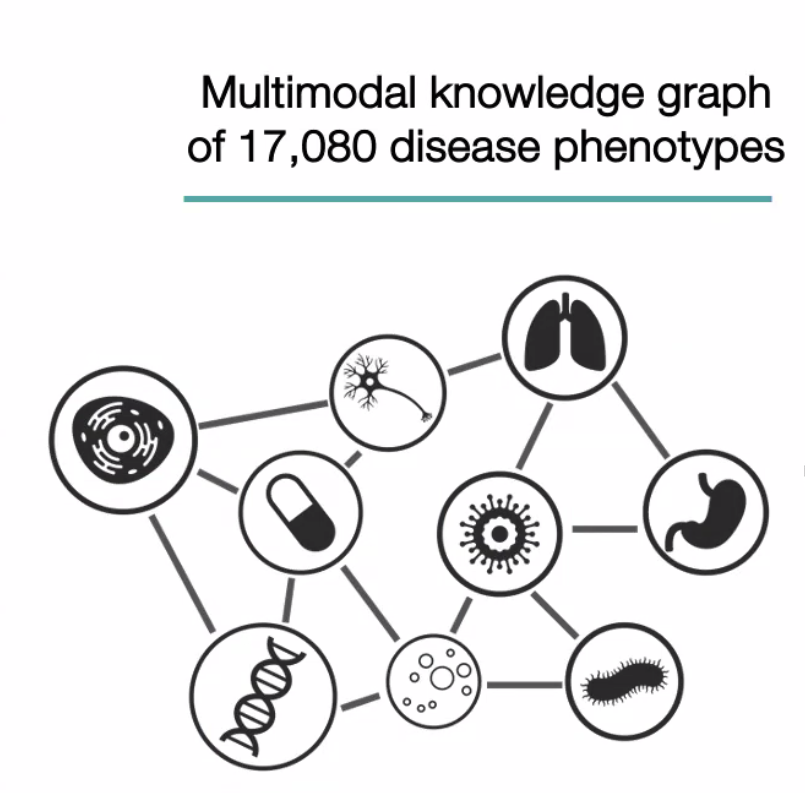
\includegraphics[scale=0.2]{MultimodalPreview.png}
    \end{figure}
    Image courtesy of partial figure from McDermott et al. {\it Structure-inducing pre-training} \cite{mcdermott_structure-inducing_2023}
\end{frame}


\begin{frame}{Molecular/Biochemical }
    \begin{figure}
        \centering
        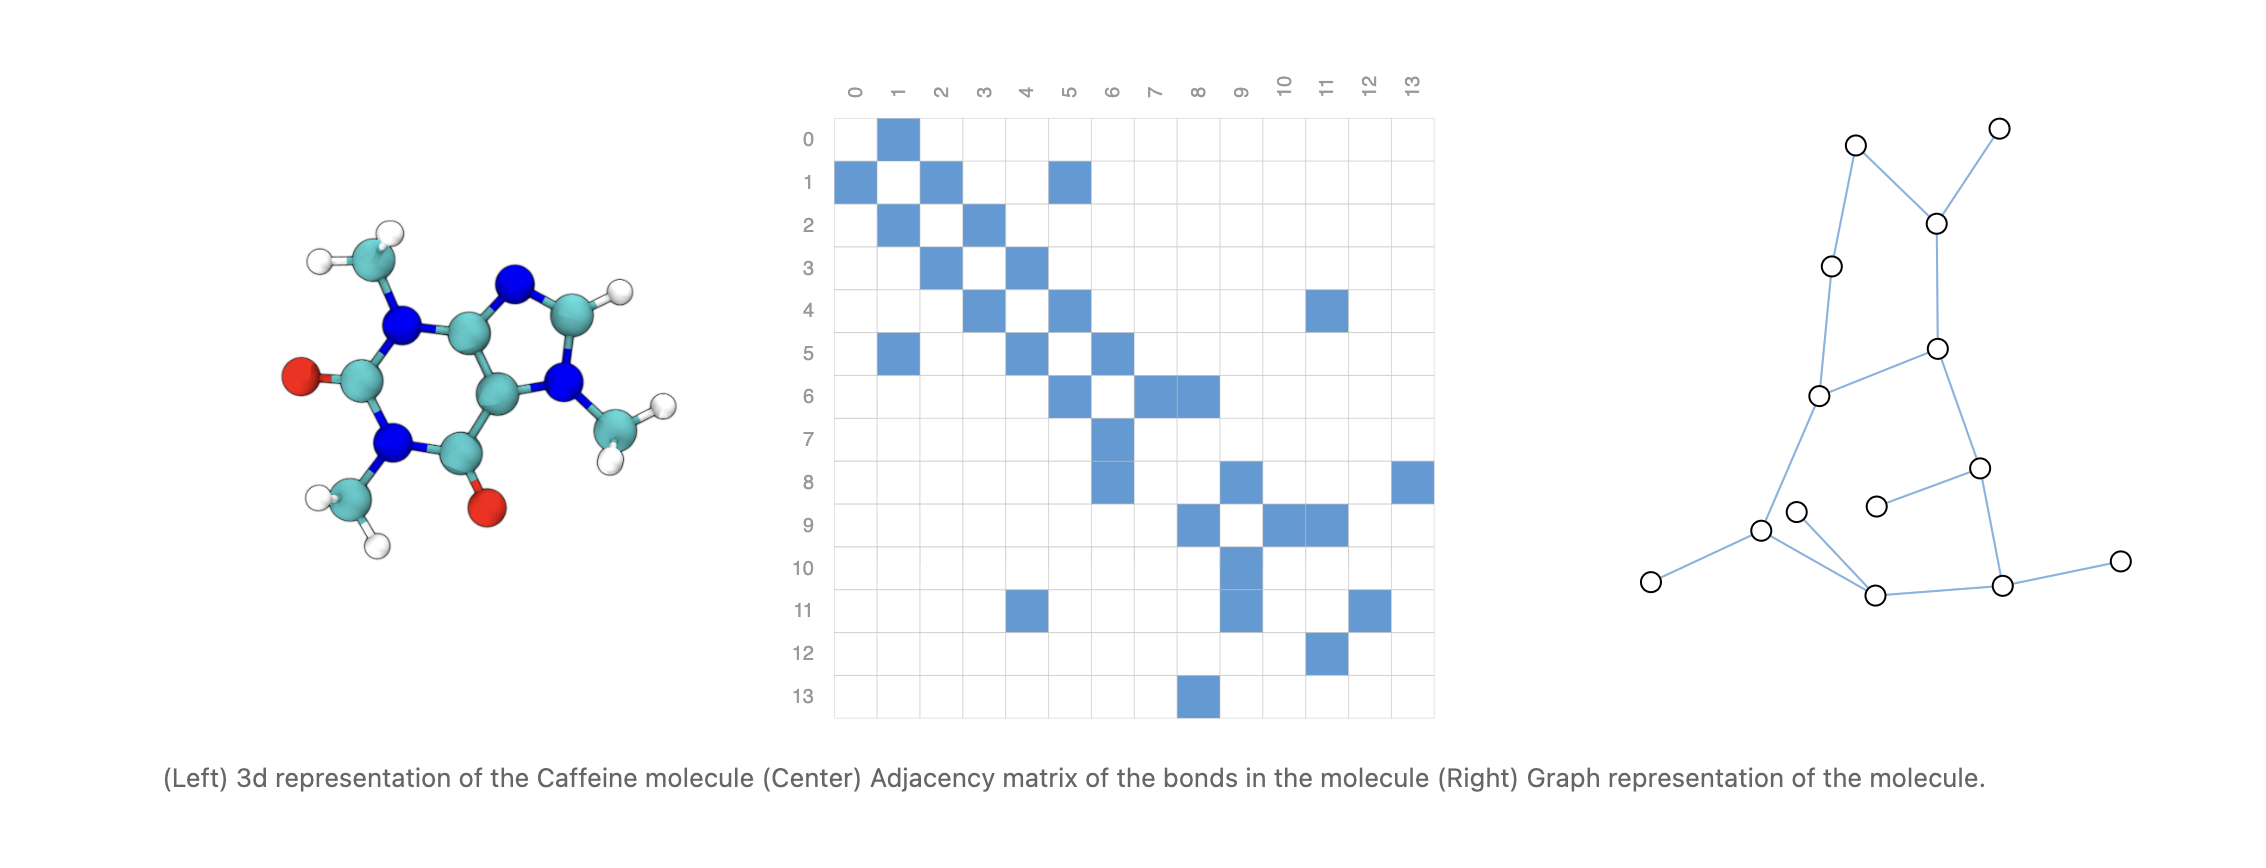
\includegraphics[scale=0.3]{Caffeine_Graph.png}
    \end{figure}
    Image courtesy of \url{https://distill.pub/2021/gnn-intro/} \cite{sanchez-lengeling_gentle_2021}
\end{frame}

\begin{frame}{Protein Representation }
    \begin{figure}
        \centering
        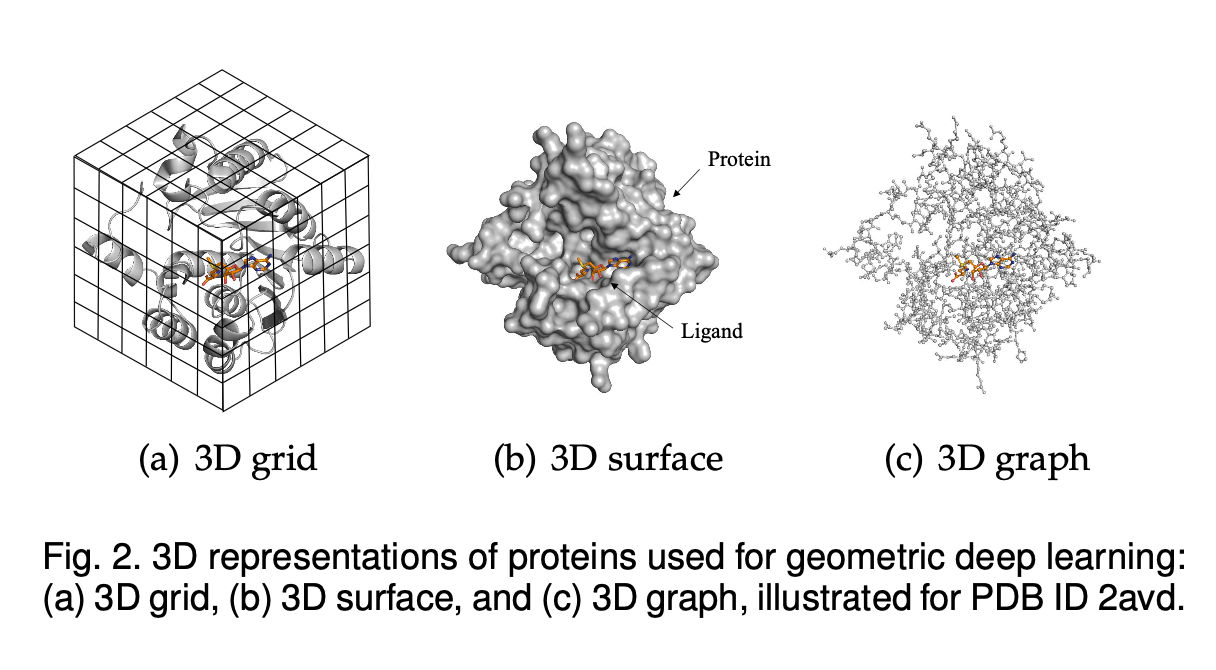
\includegraphics[scale=0.45]{Zhang_Protein3D.png}
    \end{figure}
    Fig 2. of Zhang (2023) {\it Geometric Deep Learning for Structure-Based Drug Design: A Survey} \cite{zhang_systematic_2023}
\end{frame}

\begin{frame}{Motivation}
    \begin{itemize}
        \item Want to utilize the input structure of the graph
        \begin{itemize}
            \item Respect/Maintain
            \item Update/Estimate
        \end{itemize} 
        \item "Flattening" graphical data for DNN, CNN, etc. omits useful topology from our data 
        \item Early methods attempting to retain topological info included recursive neural networks and random walk models, which GNN methodology extended \cite{scarselli_graph_2009} 
    \end{itemize}
\end{frame}



\begin{frame}{Notation/Set-Up}
    \begin{columns}[T] % align columns at the top
        \begin{column}{.7\textwidth}
            \begin{itemize}%{.5\textwidth}
                \setlength\itemsep{8mm}
%                \item Consider random vector $X \sim F(\boldsymbol\mu, \Sigma)$ and precision matrix $\Theta \equiv \Sigma^{-1}$
                \item Consider the graph $\Graph = (\NodeSet, \EdgeSet), \EdgeSet \subseteq \NodeSet \times \NodeSet$, where any node $\node$ has a related "feature vector" $x_\node \in \mathbb{R}^d$
                \begin{itemize}
                    \item Let $\NumNodes = \NumNodes$
                \end{itemize}
                \item Let $\nhood_s(\node)$ represent the $s$-hop neighborhood of any node $\node$ (and implicitly $\nhood(\node) \equiv \nhood_1(\node)$)
                \item Can construct adjacency matrix $\AdjMat \in \mathbb{R}^{\NumNodes \times \NumNodes}$ to capture structure of edge set $\EdgeSet$ 
                \begin{itemize} 
                    \item $\AdjMat_{ij}=w_{ij}\Ind\{(i,j) \in \EdgeSet\}$ for scalar weight $w_{ij} \in \mathbb{R}$
                \end{itemize}
            \end{itemize}
        \end{column}
        \begin{column}{.3\textwidth}
            %\begin{figure}
                \centering
            \scalebox{0.9}{
                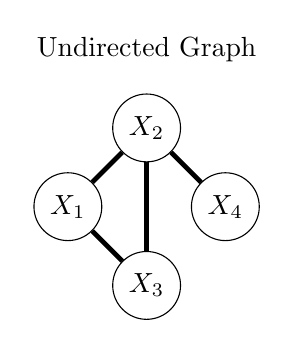
\begin{tikzpicture}
                \node[circle, draw] (A) at (0,0) {$X_1$};
                \node[circle, draw] (B) at (1,1) {$X_2$};
                \node[circle, draw] (C) at (1,-1) {$X_3$};
                \node[circle, draw] (D) at (2,0) {$X_4$};
                \node[] (capt) at (1, 2) {Undirected Graph};
                \draw[line width=0.6mm] (A) -- (B);
                \draw[line width=0.6mm] (A) -- (C);
                \draw[line width=0.6mm] (B) -- (D);
                \draw[line width=0.6mm] (C) -- (B);
            \end{tikzpicture}
            }
            %\caption{Undirected Graph}
            %\end{figure}
            \\ \vspace{3mm}
            \scalebox{0.9}{
            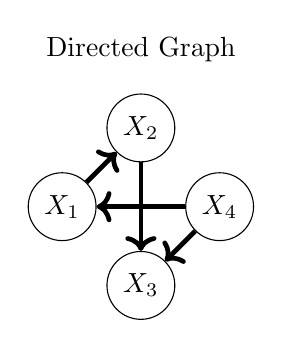
\begin{tikzpicture}%[opacity=0.2]
                \node[circle, draw] (A) at (0,0) {$X_1$};
                \node[circle, draw] (B) at (1,1) {$X_2$};
                \node[circle, draw] (C) at (1,-1) {$X_3$};
                \node[circle, draw] (D) at (2,0) {$X_4$};
                \node[] (capt) at (1, 2) {Directed Graph};
                \draw [line width=0.6mm, ->]
                    (A) edge (B)
                    (D) edge (A) 
                    (D) edge (C) 
                    (B) edge (C);
            \end{tikzpicture}
            }
        \end{column}
    \end{columns}
\end{frame}


\begin{frame}{Topology Representations}
\begin{itemize}\setlength
    \item Simplest/Na\"ive method is to use $\AdjMat$
    \item Consider also the Laplacian matrix $\LapMat = \DegMat - \AdjMat$ 
    \begin{itemize}
        \item $\mathbf{\DegMat = \text{diag}(A1_\NumNodes)}$
    \end{itemize}
    \item Can use an eigenvalue-normalized Laplacian $\LapMatNorm = \Identity - \DegMat^{-1/2}\AdjMat\DegMat^{-1/2} = \DegMat^{-1/2}\LapMat\DegMat^{-1/2}$
    \item Note that a given graph topology is represented equivalently by any permutation of its $\AdjMat$
%    \color{red}
%    \item Note on necessity of permutation invariant functions (permutations of adjacency matrix represent same graph but consistent behavior of NN/GNN is not assured by permutd A matrices)
    \end{itemize}
\end{frame}



\section{General Construction \textcolor{red}{10-20ish minutes}}
\OutlineRedux 





\begin{frame}{What do we estimate about graph structure?}
    \begin{gather*}
        \text{GNN learning can be }
        \begin{cases}
            \text{Node-wise }\Phi(\Graph, \node): (\node \in \NodeSet) \rightarrow \mathbb{R}^m 
            \\  \\ 
            \text{Edge-wise }\Phi(\Graph, \edge): (e\in \EdgeSet) \rightarrow \mathbb{R}^m  
            % can predict edge weights and prune to determine "edge presence", but I believe that GNN's take edge sets as input and preserve these edgesets 
            \\ \\ 
            \text{Graph-level characteristics }\Phi(\Graph) %\rightarrow \mathbb{R}^m 
            \end{cases}            
    \end{gather*}
\end{frame}


\begin{frame}{What do we estimate about graph structure?}
    \begin{gather*}
        \text{GNN learning can be }
        \begin{cases}
            \text{Node-wise }\Phi(\Graph, x): (x\in \NodeSet) \rightarrow \mathbb{R}^m 
            \\  \\
            \tikz[baseline]{\node[anchor=base,fill=white,inner sep=0pt,opacity=0.5] {$\text{Graph-level characteristics }\Phi(\Graph, e): (e\in\EdgeSet) \rightarrow \mathbb{R}^m$};}
            \\ \\
            \tikz[baseline]{\node[anchor=base,fill=white,inner sep=0pt,opacity=0.5] {$\text{Graph-level characteristics }\Phi(\Graph)$};} %\rightarrow \mathbb{R}^m 
        \end{cases}            
    \end{gather*}
\end{frame}


\iffalse 
                    \begin{frame}{}
                        An overly simple representation: \newline 
                        \begin{columns}[T]
                        \begin{column}{0.3\textwidth}
                            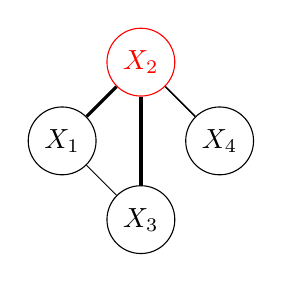
\begin{tikzpicture}
                                \node[circle, draw] (A) at (0,0) {$X_1$};
                                \node[circle, color=red, draw] (B) at (1,1) {$X_2$};
                                \node[circle, draw] (C) at (1,-1) {$X_3$};
                                \node[circle, draw] (D) at (2,0) {$X_4$};
                                \draw[line width=0.4mm] (A) -- (B);
                                \draw[line width=0.1mm] (A) -- (C);
                                \draw[line width=0.2mm] (B) -- (D);
                                \draw[line width=0.6mm] (C) -- (B);
                            \end{tikzpicture}
                        \end{column}
                        \begin{column}{0.4\textwidth}
                        % \begin{gather*}
                                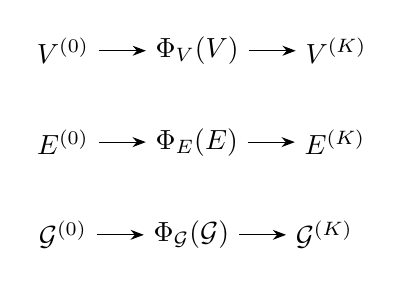
\begin{tikzpicture}[node distance=0.6cm,>=Stealth]
                                    % Nodes
                                    \node (NodeSet0) {$\NodeSet^{(0)}$};
                                    \node[right=of NodeSet0] (PhiNodeSet) {$\Phi_\NodeSet(\NodeSet)$};
                                    \node[right=of PhiNodeSet] (NodeSetIter) {$\NodeSet^{(\Iter)}$};
                                
                                    \node[below=of NodeSet0] (EdgeSet0) {$\EdgeSet^{(0)}$};
                                    \node[right=of EdgeSet0] (PhiEdgeSet) {$\Phi_\EdgeSet(\EdgeSet)$};
                                    \node[right=of PhiEdgeSet] (EdgeSetIter) {$\EdgeSet^{(\Iter)}$};
                                
                                    \node[below=of EdgeSet0] (Graph0) {$\Graph^{(0)}$};
                                    \node[right=of Graph0] (PhiGraph) {$\Phi_\Graph(\Graph)$};
                                    \node[right=of PhiGraph] (GraphIter) {$\Graph^{(\Iter)}$};
                                
                                    % Arrows
                                    \draw[->] (NodeSet0) -- (PhiNodeSet);
                                    \draw[->] (PhiNodeSet) -- (NodeSetIter);
                                
                                    \draw[->] (EdgeSet0) -- (PhiEdgeSet);
                                    \draw[->] (PhiEdgeSet) -- (EdgeSetIter);
                                
                                    \draw[->] (Graph0) -- (PhiGraph);
                                    \draw[->] (PhiGraph) -- (GraphIter);
                                \end{tikzpicture}
                        %\end{gather*}
                        \end{column}
                        \begin{column}{0.3\textwidth}
                            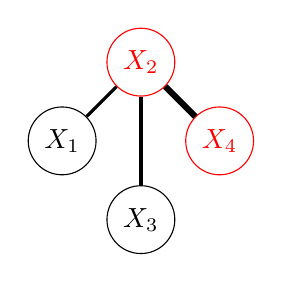
\begin{tikzpicture}
                                \node[circle, draw] (A) at (0,0) {$X_1$};
                                \node[circle, color=red, draw] (B) at (1,1) {$X_2$};
                                \node[circle, draw] (C) at (1,-1) {$X_3$};
                                \node[circle, color=red, draw] (D) at (2,0) {$X_4$};
                                \draw[line width=0.4mm] (A) -- (B);
                                %\draw[line width=0.1mm] (A) -- (C);
                                \draw[line width=0.8mm] (B) -- (D);
                                \draw[line width=0.5mm] (C) -- (B);
                            \end{tikzpicture}
                        \end{column}
                        \end{columns}

                    \end{frame}

\fi


\begin{frame}{
    General Framework\footnote{See \cite{ektefaie_multimodal_2023,gilmer_neural_2017, xu_how_2019}}
    }

    We begin with the general Message Passing Neural Networks (MPNN) structure of a GNN: 

    \vspace{4mm}
    
    \begin{algorithmic}[1]
    \State Initialize $\nrepresent^{(0)} \gets x_\node, \forall \node \in \NodeSet$ 
        \For{$\iter = 0, ..., \Iter$}:
            \For{$\node \in \Graph$}:
            \State $m_u^{(\iter+1)} \gets \text{\textcolor{blue}{Message}}(h_\node, h_u, \edge_{\node u}), \forall u \in \nhood_\node$
            \State $\nrepresent_{agg}^{(\iter+1)} \gets \text{\textcolor{blue}{Aggregate}}(\{m_u^{(\iter)} \mid u \in \nhood_\node\})$ 
            \State $\nrepresent^{(\iter+1)} \gets \text{\textcolor{blue}{Update}}(\nrepresent^{(\iter)}, \nrepresent_{agg}^{(\iter)})$
            \EndFor
        \EndFor
        \State $\hat{y} \gets \text{\textcolor{blue}{Transform}}(\{h^\Iter_\node | \node \in \Graph\})$ 
        \qquad{\hspace{4mm} or \textcolor{blue}{Readout$(\cdot)$}}
    \end{algorithmic}   

\end{frame}




\begin{frame}{General Framework}
Can succinctly represent the $\iter$th layer as: 
\begin{align*}
\iffalse 
    \mathbf{h}_\node^{(\iter+1)} 
    &=
    \text{Update}
    \left\{ 
    x_\node^{(\iter)}
    ,   
    \text{Aggregate}
    \left[
        \text{Message}
        \left(
        h_\node^{(\iter)}, x_u^{(\iter)}, \edge_{u,\node}^{(\iter)}
        \right)
    \right]
    \right\}
\\
\fi
    \mathbf{h}_\node^{(\iter+1)} 
    &=
    Up
    \left\{ 
    x_\node^{(\iter)}
    ,   
    Agg
    \left[
        Msg
        \left(
        h_\node^{(\iter)}, x_u^{(\iter)}, \edge_{u,\node}^{(\iter)}
        \right)
    \right]
    \right\}
\end{align*}

Choices of (differentiable) functions for Aggregate, Update, and Readout determine the architecture of your GNN 

\vspace{4mm}

Trained end-to-end via backpropagation for problem-specific Transform function 

\end{frame}

\begin{frame}{Aggregate \& Update}
    \begin{itemize}
        \item {\bf Aggregate$(\cdot)$} produces a representation of information from a node's neighborhood via {\bf permutation invariant} function
        \item Can include weights (edge-wise or learned)
        \item Over later iterations, this includes information from further and further distant nodes to any one target node 
        \item We then {\bf Update$(\cdot)$} our current state using this aggregated neighborhood-level information
    \end{itemize}
\end{frame}


\begin{frame}{Transform/Readout}
    \begin{itemize}
        \item {\bf Transform$(\cdot)$ } translates our learned node representations to some desired outcome 
        \begin{itemize}
            \item Regression
            \item Binary/Multi-class classification 
            \item MLP/DNN's 
        \item {\bf Readout$(\cdot)$} is common term for translating node-level output to graph-level
            \item {\it Global Pooling} - Methods applied over entire graph (e.g. averaging, fitting "regular" deep neural network, etc.)
        \end{itemize}
    \end{itemize}
\end{frame}



\begin{frame}{Graph Convolutional Network}
    \begin{itemize}
    \item Proposed in 2017 by Thomas Kipf, Max Welling \cite{kipf_semi-supervised_2017}, can consider one example of "Laplacian-based methods" \cite{gilmer_neural_2017} 
    \end{itemize}
    
        \begin{align*}
        \iffalse
            \mathbf{\nrepresent}_\node^{(\iter+1)} 
            &=
            \text{Update}
            \left( 
            x_\node^{(\iter)}
            ,   
            \text{Aggregate}
            (
                \nrepresent_\node^{(\iter)}, x_u^{(\iter)}, \edge_{u,\node}^{(\iter)}
            )
            \right)
        \\
        \fi 
            \NodeRepMat^{(\iter+1)} 
            &=
            \ReLu
            \left( 
                \mathbf{
                %D^{-1/2}
                %(\AdjMat + I)
                %D^{-1/2}
                \widetilde{\DegMat}^{-1/2}
                \widetilde{\AdjMat}
                \widetilde{\DegMat}^{-1/2}  
                \NodeRepMat^{(\iter)}
                \Theta 
                }            
            \right)
    \end{align*}
    
    \begin{itemize}
        \item Motivated by considering the graph convolution\footnote{$U$ the matrix of eigenvectors of $\LapMat$} $x \star g = UgU^Tx$ as the message passing function 
        \item Learned weight/parameter matrix $\boldsymbol\Theta$
        %\item $\mathbf{D}_{ii} = \sum_{j}\mathbf{(\AdjMat+I)_{ij}}$
        %\item Eigenvalue normalizing $\mathbf{D^{-1/2}(\AdjMat + I)D^{-1/2}}$ for computational stability
    \end{itemize}
%    \textcolor{red}{Review paper, comment on applications briefly (KG setting), also motivate through graph convolutions?}
    \end{frame}



\begin{frame}{Graph Convolutional Network}
    \begin{itemize}
    \item Proposed in 2017 by Thomas Kipf, Max Welling \cite{kipf_semi-supervised_2017}, can consider one example of "Laplacian-based methods" \cite{gilmer_neural_2017} 
    \end{itemize}
    
    \begin{align*}
        \iffalse
            \mathbf{\nrepresent}_\node^{(\iter+1)} 
            &=
            \text{Update}
            \left( 
            x_\node^{(\iter)}
            ,   
            \text{Aggregate}
            (
                \nrepresent_\node^{(\iter)}, x_u^{(\iter)}, \edge_{u,\node}^{(\iter)}
            )
            \right)
        \\
        \fi 
            \NodeRepMat^{(\iter+1)} 
            &=
            \underbrace{\ReLu}_{\text{Update}}
            \underbrace{
            \left( 
                \mathbf{
                %D^{-1/2}
                %(\AdjMat + I)
                %D^{-1/2}
                \widetilde{\DegMat}^{-1/2}
                \widetilde{\AdjMat}
                \widetilde{\DegMat}^{-1/2}  
                \NodeRepMat^{(\iter)}
                \Theta 
                }            
            \right)
            }_{\text{Aggregate/Message}}
    \end{align*}
    
    \begin{itemize}
        \item Motivated by considering the graph convolution\footnote{$U$ the matrix of eigenvectors of $\LapMat$} $x \star g = UgU^Tx$ as the message passing function 
        \item Learned weight/parameter matrix $\boldsymbol\Theta$
        %\item $\mathbf{D}_{ii} = \sum_{j}\mathbf{(\AdjMat+I)_{ij}}$
        %\item Eigenvalue normalizing $\mathbf{D^{-1/2}(\AdjMat + I)D^{-1/2}}$ for computational stability
    \end{itemize}
%    \textcolor{red}{Review paper, comment on applications briefly (KG setting), also motivate through graph convolutions?}
    \end{frame}



\begin{frame}{Graph Convolutional Network}
    \textcolor{red}{Maybe move to appendix} \\ 
Intuitive "derivation": 
\begin{align*}
    \NodeRepMat^{(\iter+1)}
    &=
    \sigma
    \left( 
        \AdjMat \NodeRepMat^{(\iter)} \Theta
    \right) 
\\
    \NodeRepMat^{(\iter+1)}
    &=
    \sigma
    \left( 
        \DegMat^{-1}\AdjMat \NodeRepMat^{(\iter)} \Theta
    \right) 
    \qquad{\text{Normalizing by degree}}
\\
    \NodeRepMat^{(\iter+1)}
    &=
    \sigma
    \left( 
        \DegMat^{-1/2}\AdjMat\DegMat^{-1/2} \NodeRepMat^{(\iter)} \Theta
    \right) 
    \qquad{\text{Symmetric normalization}} % "no longer simple averaging"
\\
    \NodeRepMat^{(\iter+1)}
    &=
    \sigma
    \left( 
        \widetilde{\DegMat}^{-1/2}
        \widetilde{\AdjMat}
        \widetilde{\DegMat}^{-1/2} \NodeRepMat^{(\iter)} \Theta
    \right) 
    \qquad{\text{Adding self-loop}}
\end{align*}

where $\widetilde{\AdjMat} = \AdjMat + \Identity, \widetilde{\DegMat}_{ii} = \sum_j \widetilde{\AdjMat}_{ij}$, $\sigma$ is any activation function, $\NodeRepMat$ is simply the matrix of $\mathbf{\nrepresent}_\node$ for all nodes 
% intuition here is normalizing by a nodes degree (left mult) and "averaging" neighborhood degree (right mult)
% nice explainer \url{https://math.stackexchange.com/questions/3035968/interpretation-of-symmetric-normalised-graph-adjacency-matrix}
\end{frame}


\begin{frame}{General Framework (Revisited)}
    \begin{itemize}\setlength\itemsep{8mm}
        \item {\bf Input} 
            \begin{itemize}
                \item Node conceptualization
                \item Node embeddings
            \end{itemize}
        \item {\bf Architecture}
            \begin{itemize}
                \item $\NodeRepMat^{(\iter+1)} 
                =
                \ReLu
                \left( 
                    \mathbf{
                    %D^{-1/2}
                    %(\AdjMat + I)
                    %D^{-1/2}
                    \widetilde{\DegMat}^{-1/2}
                    \widetilde{\AdjMat}
                    \widetilde{\DegMat}^{-1/2}  
                    \NodeRepMat^{(\iter)}
                    \Theta 
                    }            
                \right)$
            \end{itemize}
        \item {\bf Output}
            \begin{itemize}
                \item Target output (Readout, Transform functions)
                \item Loss function
            \end{itemize}
\end{itemize}
\end{frame}




\section{Applications and Extensions \textcolor{red}{20-25ish minutes}}
\OutlineRedux



\subsection{Multimodal Graph Learning (MGL)}

\begin{frame}{}
    \bf{\Large Multimodal Graph Learning (MGL)}    
\end{frame}

\begin{frame}{Multimodal Graph Learning (MGL)}
\begin{itemize}\setlength\itemsep{6mm}
    \item Ektefaie (2023) {\it Multimodal learning with graphs} \cite{ektefaie_multimodal_2023}
    \item \textcolor{red}{Cite 14-16 in multimodal paper for multi improvement over uni VAE} 
    \item Topology is complicated by multimodality of input data 
    \begin{itemize}
        \item Modal collapse \cite{javaloy_mitigating_2022}
        \item Differential data availability 
        \item \textcolor{red}{Can mention Kipf algorithm does well in semi-supervised setting (even with limited labels available within a given "cluster"), so if we have some gold standard data (biomarker/strong proxy, etc.) that is difficult to obtain, can be VERY useful to include for MGL and lead to good performance, no bullet point here just mention}
    \end{itemize}
\end{itemize}    

\end{frame}

\begin{frame}{Mutimodal}
    \begin{columns}[T]
        \begin{column}{0.5\textwidth}
            Clinical Data
            \begin{itemize}        
                \item Clinical text  
                \item -omics data 
                \item Laboratory measurements 
                \item Clinical imaging
            \end{itemize}
            \end{column}
        \begin{column}{0.5\textwidth}
            Protein Structures
            \begin{itemize}        
                \item 1$^\circ$ AA Sequence
                \item 2$^\circ$ Helix interactions
                \item 3$^\circ$ Folding, bridges 
            \end{itemize}
        \end{column}
%        \begin{column}{0.3\textwidth}
%            Text Data
%            \begin{itemize}        
%                \item 
%            \end{itemize}
%        \end{column}
    \end{columns}
\end{frame}


\begin{frame}{Framework}
    Authors propose a four component "blueprint"
    \begin{enumerate}
    \item Identifying entitites (i.e. modalities)
    \item Uncovering topology 
    \begin{itemize}
        \item {\it A priori}
        \item Adaptively learned
    \end{itemize}
    \item Propagating information 
    \item Mixing representation 
    \end{enumerate}
\end{frame}


\begin{frame}{Framework}
    Authors propose a four component "blueprint"
    \begin{enumerate}
    \item Identifying entitites (i.e. modalities)
    \item Uncovering topology 
    \item {\bf Propagating information }
    \item {\bf Mixing representation }
    \end{enumerate}
    \begin{tikzpicture}[overlay,remember picture]
        \draw[decorate,decoration={calligraphic brace, amplitude=4pt},line width=1.2pt]
        (6.7,2.6) -- (6.7,1.7) node[midway, right=6pt, xshift=-2pt, text=black] {\footnotesize Structure Learning};
    \end{tikzpicture}

    \begin{tikzpicture}[overlay,remember picture]
        \draw[decorate,decoration={calligraphic brace, amplitude=4pt},line width=1.2pt]
        (5.2,1.8) -- (5.2,0.95) node[midway, right=6pt, xshift=-2pt, text=black] {\footnotesize Learning On-Structure Phase};
    \end{tikzpicture}
\end{frame}

\begin{frame}{Structure Learning}
    \begin{columns}[T]
    \begin{column}{0.5\textwidth}
        \vspace{12mm}
        \begin{itemize}
            \item Consider patients as {\it nodes} 
            \item Consider modalities as {\it entities} (colored nodes)
            \begin{itemize}
                \item Clinical text/narrative data 
                \item Laboratory/Physiological measurements 
                \item Image/Video data 
                \item Patient reported measurements/symptoms
                \item etc. 
            \end{itemize}
        \end{itemize}      
    \end{column}
    \begin{column}{0.5\textwidth}
        \begin{figure}
            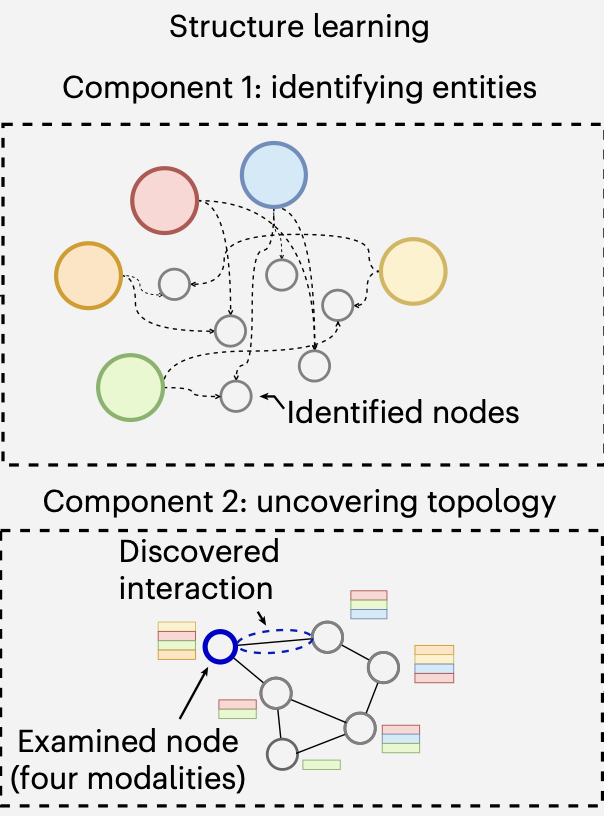
\includegraphics[scale=0.4]{Ektefaie_StructureLearning.png}
            \caption{Subset of Fig 2c \cite{ektefaie_multimodal_2023}}
        \end{figure}    
    \end{column}
\end{columns}
\end{frame}

\begin{frame}{Learning on Structure}
    
\end{frame}


\subsection{Knowledge-Graph Data}


\subsection{Structure-Based Drug Design (SBDD)}

\begin{frame}{}
    \bf{\Large Proteins and Structure-Based Drug Design (SBDD)}    
\end{frame}


\iffalse 
            \begin{frame}{AlphaFold}
                \textcolor{red}{Image and very brief acknowledgement/link for AlphaFold, ESMFold here (~30s)}
            \end{frame}
\fi 

\begin{frame}{Structure-Based Drug Design (SBDD)}
    \begin{itemize}
        \item Zhang (2023) {\it Geometric Deep Learning for Structure-Based Drug Design: A Survey} \cite{zhang_systematic_2023}
        \item SBDD aims to improve drug-discovery by understanding 3D protein structures and predicting drug efficacy/behavior % docking, conformations, etc. summarize as useful to understand behavior of drug based on target protein structure 
        \item Problems of note for GNN's include {\bf binding site prediction} and {\bf binding affinity prediction}
    \end{itemize}

    \vspace{3mm}

    \begin{columns}
        \begin{column}{0.5\textwidth}
            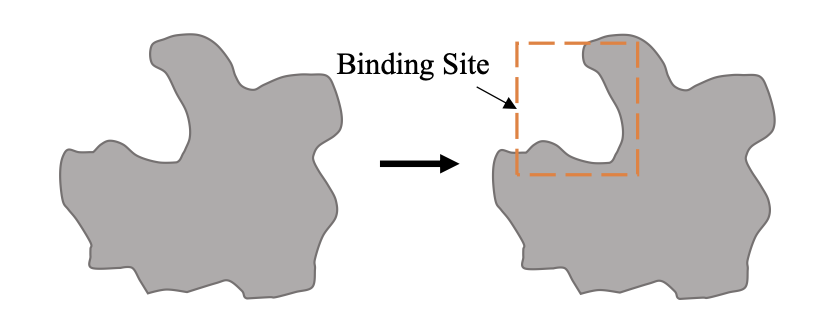
\includegraphics[width=\textwidth]{Zhang_2023_BindingSite.png}
        \end{column}
        \begin{column}{0.5\textwidth}
            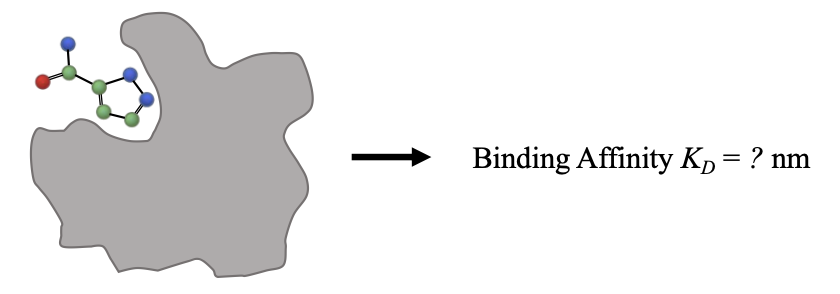
\includegraphics[width=\textwidth]{Zhang_2023_BindingAffinity.png}
        \end{column}
    \end{columns}
    \centering{\small Images from Fig. 1 of Zhang (2023) \cite{zhang_systematic_2023}}
\end{frame}

\begin{frame}{Output}
    \begin{itemize}
        \item {\bf Binding site prediction} is binary categorization at the (surface) amino acid level 
        \item {\bf Binding affinity prediction} is a continuous measure of protein-ligand interaction strength 
        \item Protein Databank (PDB), PDBBind, Dockground, CSAR-HiQ are existing data sets used to train most GNN's in these contexts 
        \item Other characteristics are important for drug design and protein-ligand interactions but without current GNN methods to my knowledge 
        \begin{itemize}
            \item Binding pose 
            \item Ligand generation 
            \item Linker design 
        \end{itemize}
    \end{itemize}
\end{frame}

\iffalse 
            \begin{frame}{Input}
                \begin{columns}
                \begin{column}{0.7\textwidth}
                \begin{itemize}\setlength\itemsep{6mm}
                    \color{red}
                    \item Nodes are radial patches (i.e. points)
                    \item Focus on complications of 3D geometry 
                    \vspace{8mm}
                    \begin{minipage}{\textwidth}
                    \item Invariant, necessary as previously stated ("coordinate system robust")
                    \item Equivariant, less strict than invariant, some transformations should generate different output (see protein conformations for drug-ligand interaction) 
                    \end{minipage}
                \end{itemize}
                \end{column}

                \begin{column}{0.3\textwidth}
                    \vspace*{-12mm}
                    %\begin{figure}
                        \begin{flushright}
                        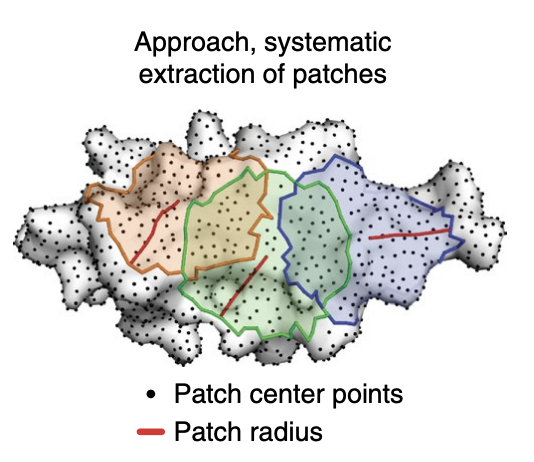
\includegraphics[width=\textwidth]{Gainza_2020_ProteinNodesRadii.png}  \\ 
                        Fig 1a. Gainza (2020) \cite{gainza_deciphering_2020}
                        \end{flushright}
                    %\end{figure}    
                \end{column}
            \end{columns}
            \end{frame}
\fi 





\begin{frame}{Input}
    \begin{figure}
        \centering 
        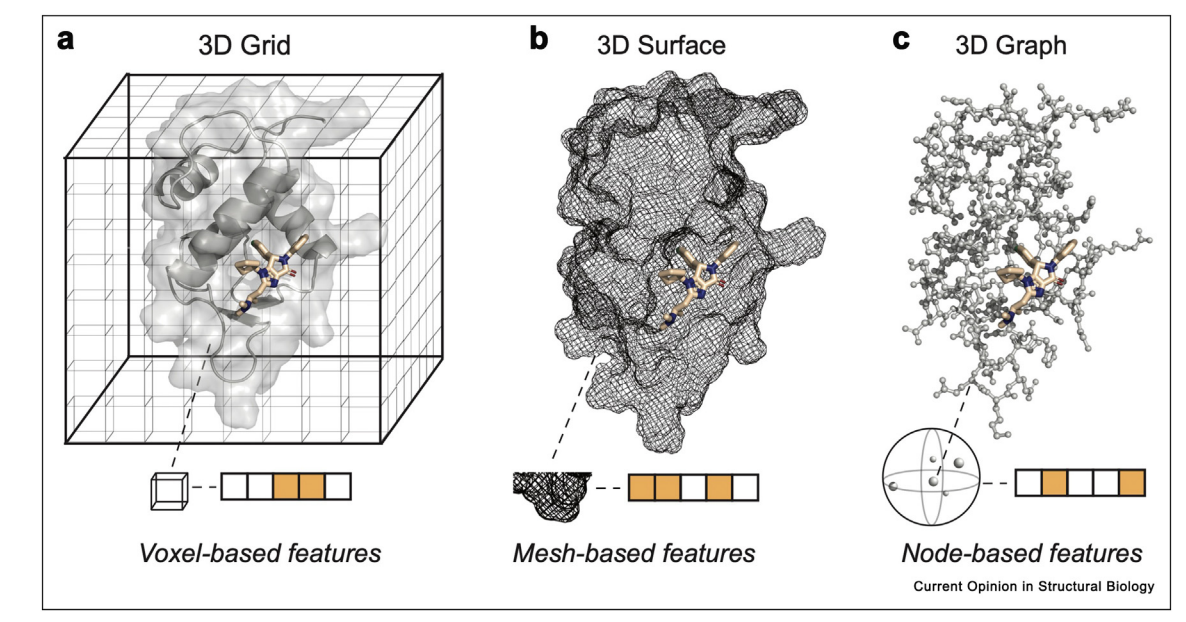
\includegraphics[scale=0.55]{Isert_2023_ModelsSBDD.png}
    \end{figure}
    Figure from Isert (2023) \cite{isert_structure-based_2023}
\end{frame}

\begin{frame}{CNN Input}
    \begin{itemize}
        \item Nodes and edges defined by radial patches about a discretization of the protein surface 
    \end{itemize}

    \begin{figure}
        \centering 
        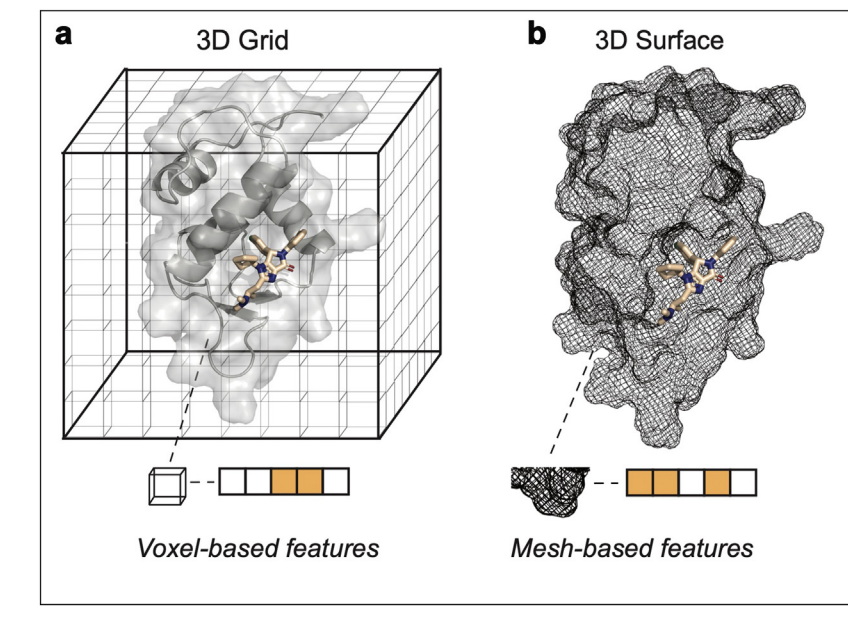
\includegraphics[scale=0.4]{Isert_2023_ModelsSBDD_VoxelMesh.png}
%    \end{figure}
%
%    \begin{figure}
%        \centering
        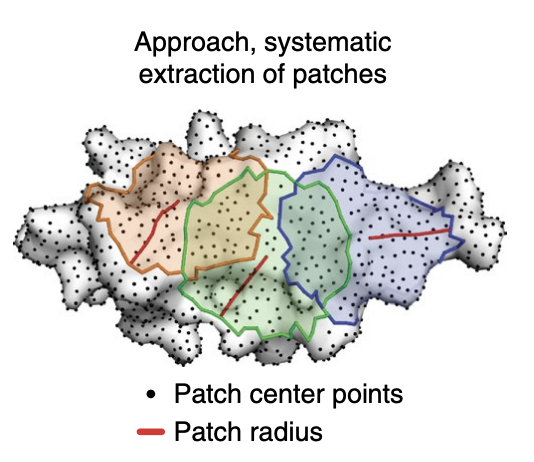
\includegraphics[scale=0.5]{Gainza_2020_ProteinNodesRadii.png}  \\ 
        Left: Fig 2(ab) from Isert (2023); Right: Fig 1a. Gainza (2020) \cite{isert_structure-based_2023, gainza_deciphering_2020}
    \end{figure}
\end{frame}



\begin{frame}{GNN Input}
    \begin{columns}
        \begin{column}{0.7\textwidth}
            \begin{itemize}
                \item Atomic structure in Euclidean space 
                \item Amino acid (also "residue") structure 
            \end{itemize}            
        \end{column}
        \begin{column}{0.3\textwidth}
            \begin{figure}
                \centering 
                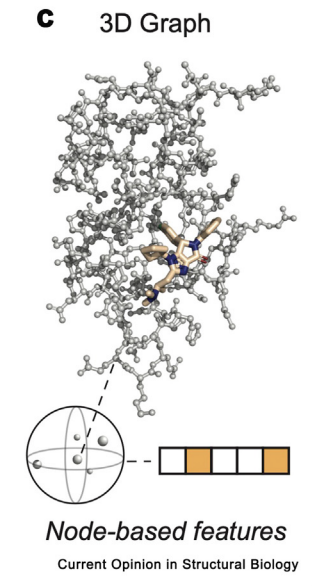
\includegraphics[scale=0.55]{Isert_2023_ModelsSBDD_3DGraph.png}
            \caption{Figure 1c from Isert (2023) \cite{isert_structure-based_2023}}
        \end{figure}
                    
        \end{column}
    \end{columns}
\end{frame}

\begin{frame}{Architecture}
Consider some transformations $T, T'$ (e.g. reflection, rotation, etc.) within the same symmetry group: \newline 
\vspace{3mm} 
\\ 

Invariance: $f(T(x)) = T'(f(x)) = f(x)$
\\
\vspace{6mm}

Equivariance: 
$\forall  T, \  \exists T': f(T(x)) = T'(f(x))$

\end{frame}

\begin{frame}{Architecture}
Forgoing the iteration supercripts, one message pass can be represented as such: 
    \begin{align*}
        m_{ij}
        &=
        \textcolor{blue}{Msg_m}(\mathbf{\node_i}, \mathbf{\node_j}, \nrepresent_i, \nrepresent_j, \edge_{ij}) 
    \\ 
        \mathbf{m}_{ij}
        &=
        Msg_{\mathbf{m}}
        (\mathbf{\node_i}, \mathbf{\node_j}, \nrepresent_i, \nrepresent_j, \edge_{ij})
    \\
        \nrepresent_i'
        &=
        \textcolor{blue}{Update_\nrepresent}
        \left[
            \nrepresent_i
            , 
            Agg_h
            (
                \{m_{ij}\}_{j \in \nhood(\node_i)}
            )
        \right]     
    \\
        \mathbf{\node_i'}
        &=
        Update_{\mathbf\node}
        \left[
            \mathbf{\node}_i
            Agg_\mathbf{\node}
            \left( 
                \{\mathbf{m}_{ij}\}_{j \in \nhood(\node_i)}
            \right)
        \right]
    \end{align*}

    where \textcolor{blue}{$Msg_m, Update_h$} are geometrically {\bf invariant}, scalar functions and $Msg_{\mathbf{m}}, Update_{\mathbf\node}$ are geometrically \bf{equivariant}, vector functions \newline 
    Here $\mathbf\node \in \mathbb{R}^3$ are 3-D coordinates (e.g. atom or amino acid location)
\end{frame}

\begin{frame}{Equivariant GNN's}
\textcolor{red}{Recreate message passing for equivariant GNN's with my notation for consistency, emphaseize new equivariant vector functions}
\begin{align*}
    h_{ij}^{(\iter)}
    &=
    \Agg(\mathbf{\node}_i, )
\end{align*}
\end{frame}

\begin{frame}{Specific GNN Implementation}
    \textcolor{red}{Review/cite one of the eGNN's from the Zhang paper}
\end{frame}



\section*{Conclusion}

\begin{frame}{}
    \bf{\LARGE Conclusion}    
\end{frame}



\begin{frame}[allowframebreaks]{References}
    \begin{itemize}
    \item Some diagrams generated in conjunction with ChatGPT 3.5
    \end{itemize}
    \printbibliography 
\end{frame}


%%%%%%%%%%%%%%%%%%%%%%%%%%
%%%%%%%%%%%%%%%%%%%%%%%%%%
% Appendix 
%%%%%%%%%%%%%%%%%%%%%%%%%%
%%%%%%%%%%%%%%%%%%%%%%%%%%

\section*{Appendix}

\begin{frame}{}
\bf{\LARGE Appendix Slides}    
\end{frame}

\begin{frame}{Implementations}
    \begin{itemize}
        \item \href{https://pytorch-geometric.readthedocs.io/en/latest/}{PyTorch Geometric} with directed extension \href{https://github.com/SherylHYX/pytorch_geometric_signed_directed}{PyTorch Geometric Signed Directed}
        \item \href{https://github.com/tensorflow/gnn}{TensorFlow GNN} \cite{ferludin_tf-gnn_2023}
        \item \href{https://carlolucibello.github.io/GraphNeuralNetworks.jl/dev/}{GraphNeuralNetworks.jl}
        \item \href{https://graphneural.network/}{Spektral}, Keras-based Pythhon package 
        \item Limited but some implementation in R 
        \begin{itemize}
            \item \href{https://cran.r-project.org/web/packages/scapGNN/vignettes/vignette.html}{scapGNN}, package GNN implementation but specific/narrow for single-cell -omics data 
        \end{itemize}
    \end{itemize}
\end{frame}

\begin{frame}{Abbreviated History}
    \begin{itemize}
        \item Graph Neural Network first(?) coined in Gori (2005) \cite{gori_new_2005} and subqeuently in Scarselli (2009) {\it The Graph Neural Network Model} \cite{scarselli_graph_2009}
        \item Graph Convolutional Network by Kipf (2017) \cite{kipf_semi-supervised_2017} but with similar convolutional message-passing algorithms (within GNN's) proposed in at least 2015 \cite{duvenaud_convolutional_2015}
        \item Message passing GNN proposed in Gilmer (2017), applications in molecular chemistry \cite{gilmer_neural_2017} 
    \end{itemize}
\end{frame}

\begin{frame}[allowframebreaks]{Additional Applications, Interesting Papers}
    \begin{itemize}
        \item Applications in travel time prediction, 2021 (\url{https://arxiv.org/pdf/2108.11482.pdf})
        \item Someone has compiled graph-/GNN-relevant talks for NeurIPS 2023 at \url{https://github.com/XiaoxinHe/neurips2023_learning_on_graphs}
    \end{itemize}
\end{frame}

\begin{frame}{DiffPool}
    Figure 1 from Ying (2018) {\it Hierarchical Graph Representation Learning with Differentiable Pooling} \cite{ying_hierarchical_2018}
    \begin{figure}
        \centering 
        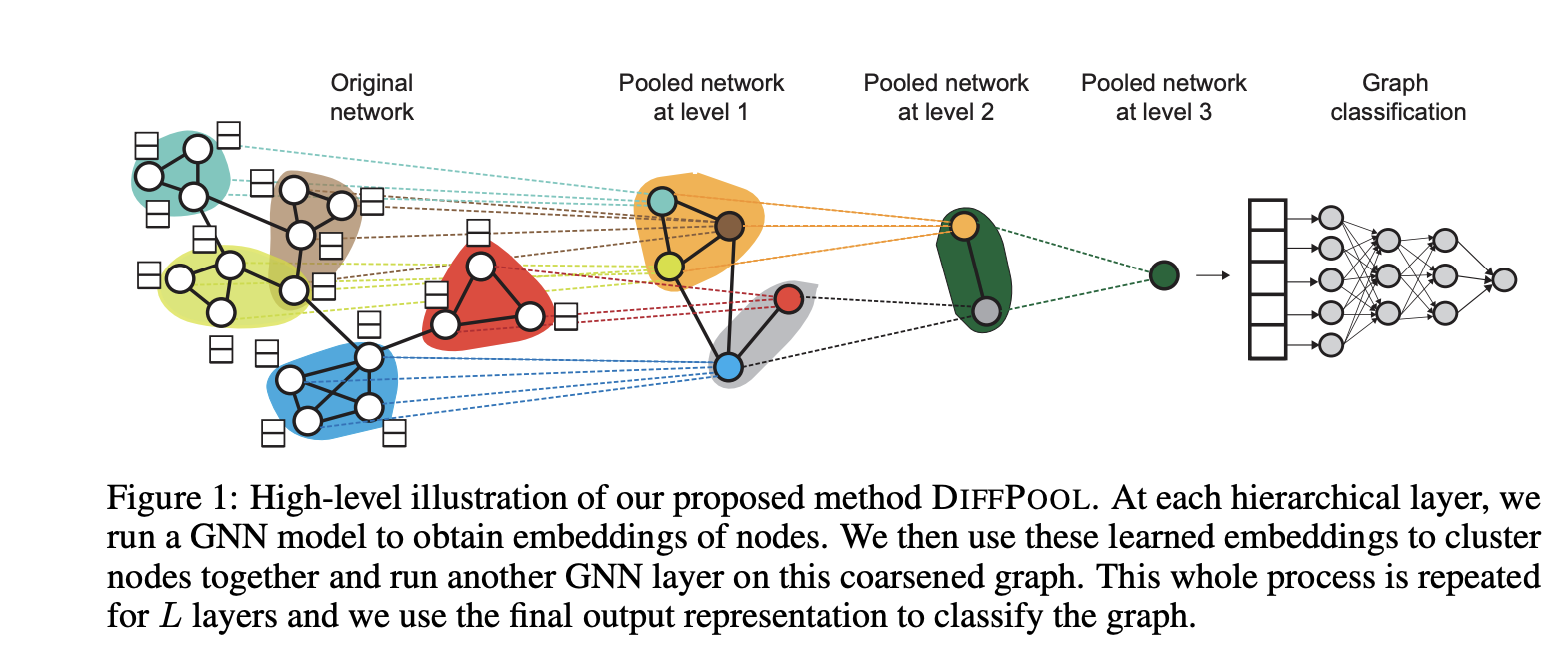
\includegraphics[scale=0.45]{DIFFPOOL_RexYing.png}
    \end{figure}
\end{frame}

\begin{frame}{KG AI Models}
    Full figure from McDermott et al. \cite{mcdermott_structure-inducing_2023}, cropped and presented in Introduction:
    \begin{figure}
        \centering
        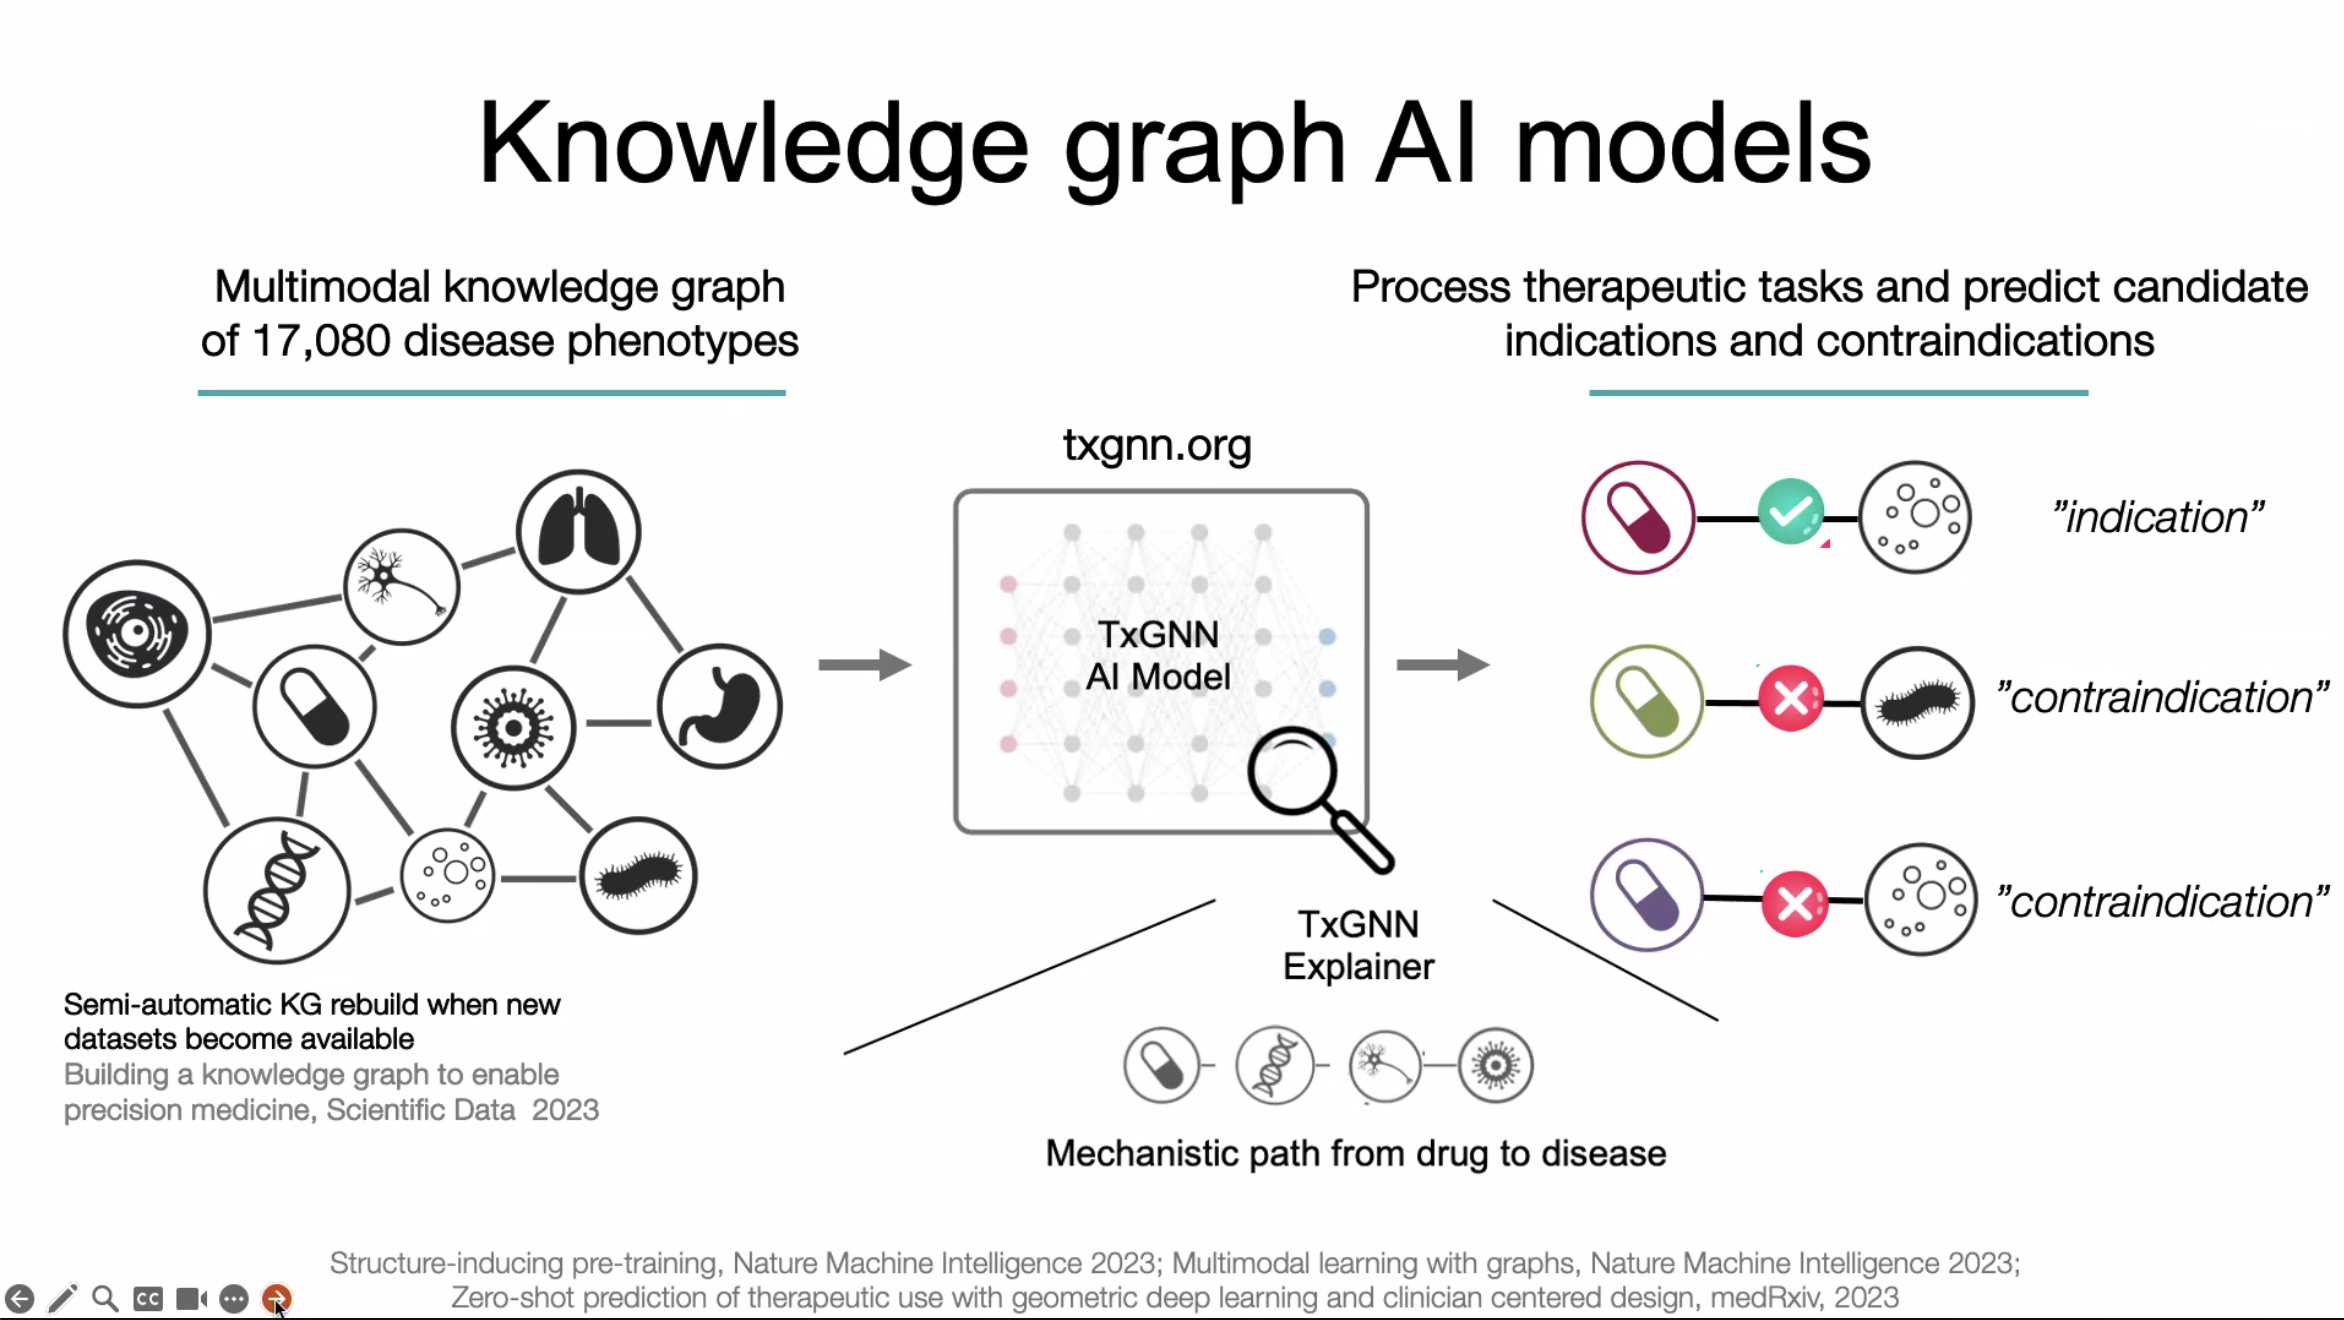
\includegraphics[scale=0.13]{Junwei_KG_Models_Infograph.png}
    \end{figure}
\end{frame}

\begin{frame}{Protein Data Bank File}
    \begin{figure}
        \centering
        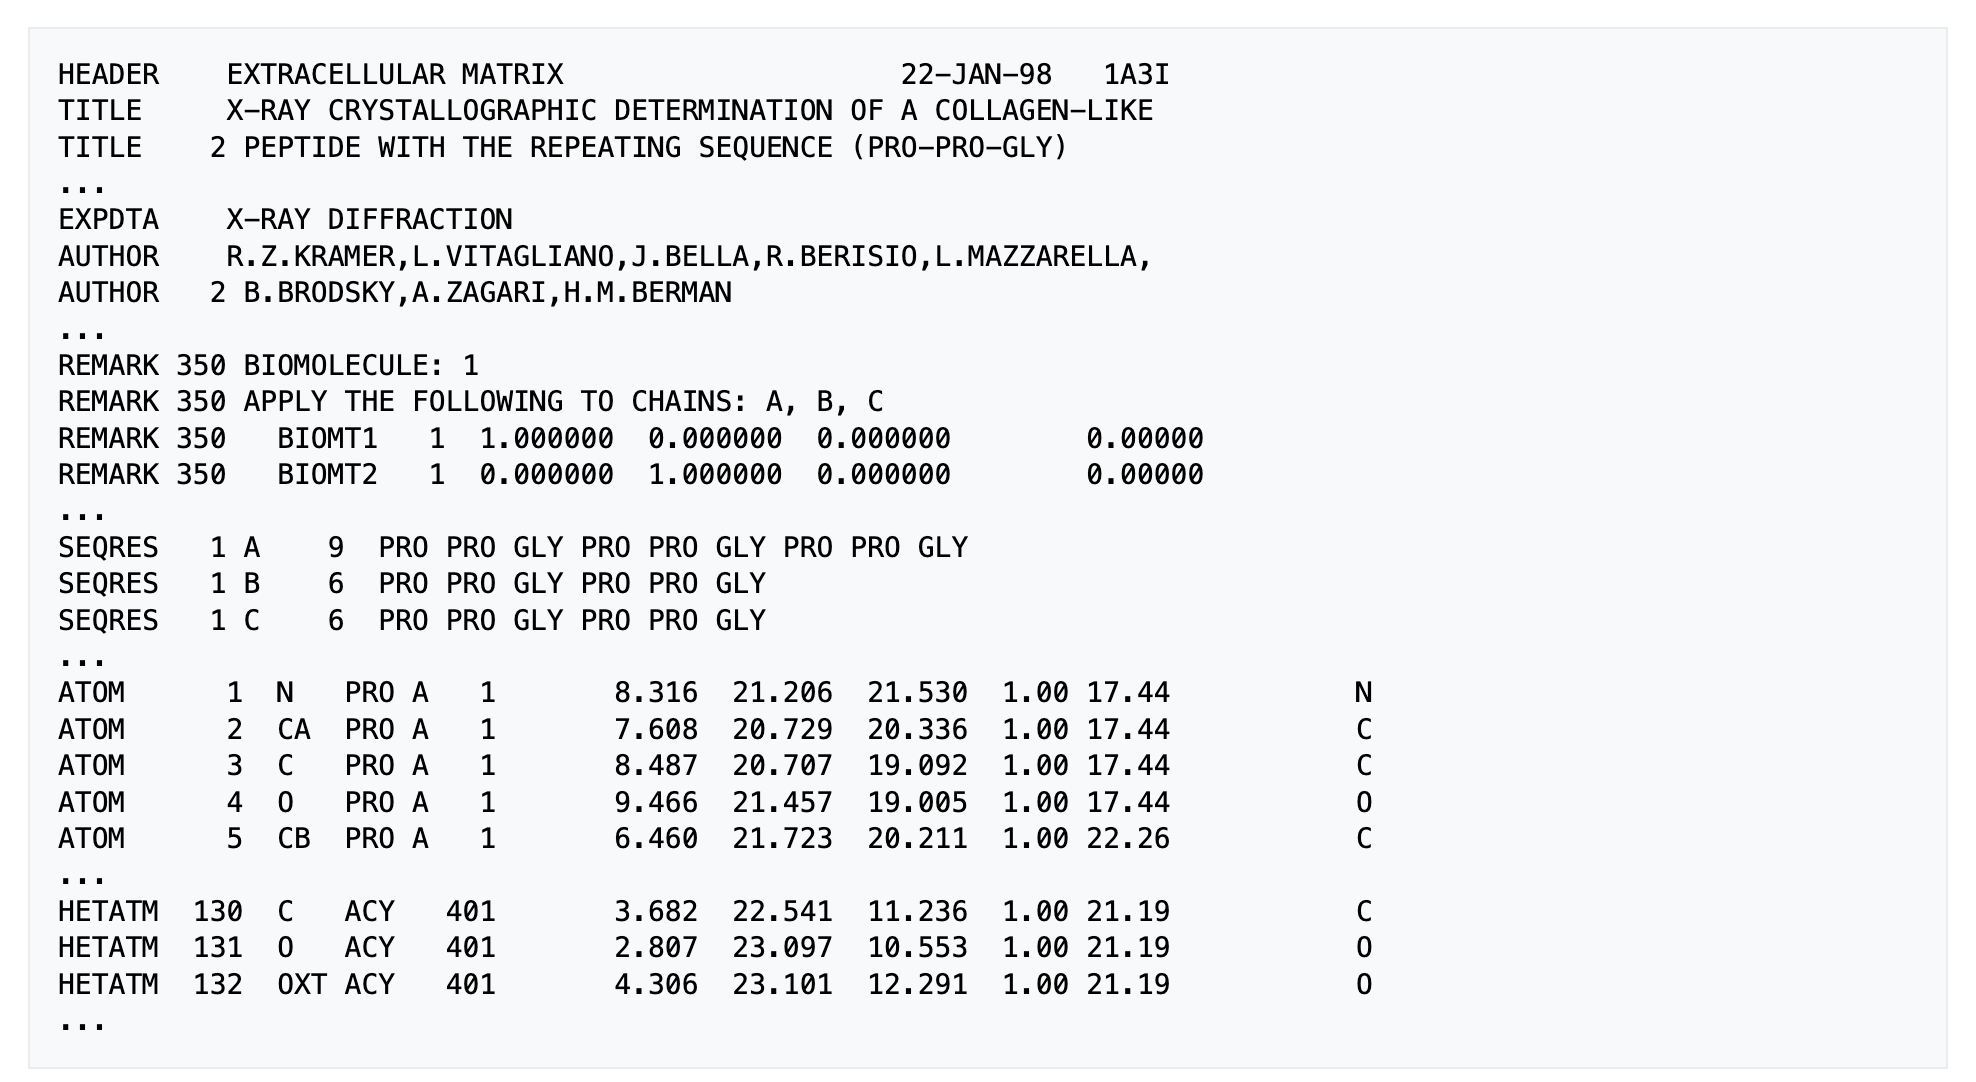
\includegraphics[scale=0.37]{PDB_File_Ex.png}
        \caption{Example PDB file structure/protein information. Taken directly from Wikipedia: \url{https://en.wikipedia.org/wiki/Protein_Data_Bank_(file_format)}
        }
    \end{figure}
\end{frame}
\end{document}